\documentclass[xcolor={table}]{beamer}
\usepackage[english]{babel}
\usepackage[utf8]{inputenc}

\usepackage{hyperref}
\usepackage{url}
\usepackage{amsmath}
\usepackage{graphicx}
\usepackage{animate}
\usepackage{enumerate}
\usepackage{subcaption}
\usepackage{multicol}
\usepackage[full, italic, slant]{complexity}
\usepackage{appendixnumberbeamer}

\usepackage[T1]{fontenc}
\usepackage{color}
\usepackage{stmaryrd}
\usepackage{amsmath} 
\usepackage{amsthm}
\usepackage{listings}
\usepackage{caption}
\usepackage{subcaption}
\usepackage{float}
\usepackage{algorithm2e}
\usepackage{hyperref}
\usepackage{booktabs}
\usepackage{indentfirst}




\expandafter\def\expandafter\insertshorttitle\expandafter{%
  \insertshorttitle\hfill\insertframenumber\,/\,\inserttotalframenumber}

\def\*{{\bf FIXME: }}

\setbeamertemplate{caption}[numbered]
\setbeamertemplate{bibliography item}{\insertbiblabel}
\newtheorem{deff}{Definícia}[section]

\mode<presentation> {
    \usetheme{Warsaw}
    \usecolortheme{seahorse}
    \usecolortheme{rose}
    \usefonttheme{professionalfonts}
    \setbeamercovered{transparent}
}

\definecolor{bloodred}{RGB}{200,0,0}


\title[eLSA]{Improving LSA word weights for document classification}

\author[Macko, Malinovska] % (optional, for multiple authors)
{Bc. Vladimír Macko\inst{1} \\ \and {\small supervisor: RNDr. Kristína Malinovská, PhD.\inst{1}}}
 
\institute[VFU] % (optional)
{
  \inst{1}%
  Comenius University\\
  Faculty of Mathematics, Physics and Informatics
}


\begin{document}
        
\begin{frame}
    \titlepage
\end{frame}
    
\begin{frame}{Overview}
    \begin{block}{}
        \begin{itemize}
            \item Introduction
            \item Problem outline
            \item Our work
            \item Results
        \end{itemize}
    \end{block}
\end{frame}

%%%%%%%%%%%%%%%%%%%%%
\section{Introduction}
\begin{frame}{Document classification}
    \begin{block}{Sentiment analysis}
        \emph{This was a terrible movie} $=$ negative sentiment
    \end{block}
    
    \begin{block}{}   
        \begin{itemize}
            \item create representation for words
            \item create representation for document
            \item predict
            %\item small, specific datasets
        \end{itemize}
    \end{block}
\end{frame} 

\begin{frame}{LSA}
    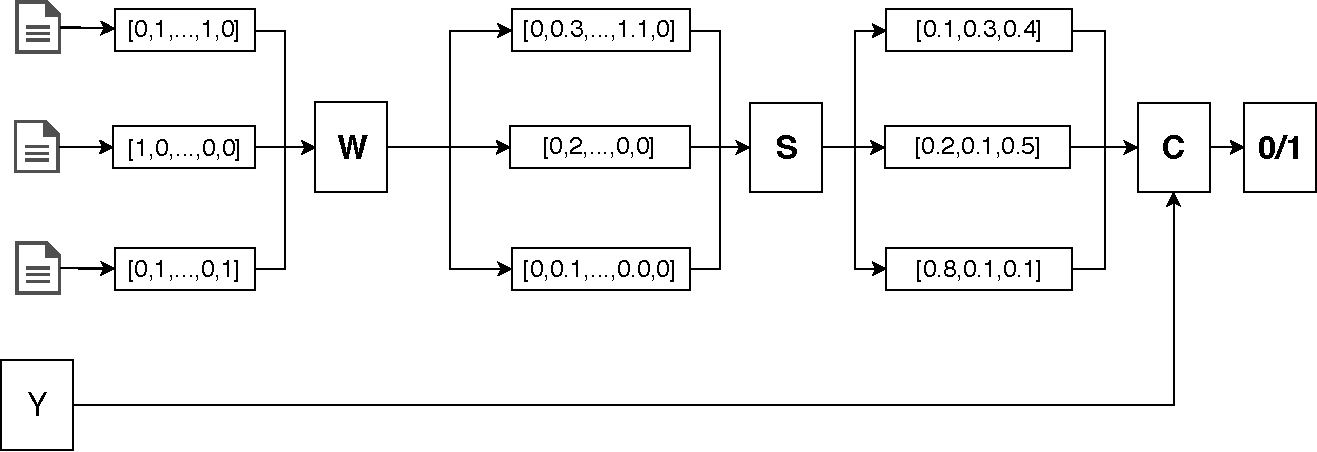
\includegraphics[width=0.9\textwidth]{LSA.pdf}
    \begin{block}
        
        $W$: reweighting

        $S$: decomposition
        
        $C$: classifier
    \end{block}
\end{frame}

\begin{frame}{SVD}
~
    {\tiny $$
\begin{matrix} 
 M &  ~~ U & \Sigma & V^T \\
 \textbf{t}_j^T &  & &  \\
 \downarrow &  & &  \\
(\textbf{d}_i) \rightarrow 
\begin{bmatrix}
x_{1,1} \dots  x_{1,n} \\
\vdots ~~~  \ddots ~~~ \vdots \\
x_{i,1} \dots  x_{i,n} \\
\vdots ~~~ \ddots ~~~ \vdots \\
x_{m,1} \dots  x_{m,n} \\
\end{bmatrix}
=
&
\textbf{u}_i \rightarrow
\begin{bmatrix} 
\begin{bmatrix} & \textbf{u}_1 & \end{bmatrix} \\
\vdots \\
\begin{bmatrix} & \textbf{u}_m & \end{bmatrix}
\end{bmatrix}
&
\cdot
\begin{bmatrix} 
\sigma_1 \dots ~~~ 0 \\
\vdots ~~~ \ddots  \vdots \\
0  \dots  \sigma_l \\
\end{bmatrix}
&
\cdot
\begin{bmatrix} 
\begin{bmatrix} \, \\ \, \\ \textbf{v}_1 \\ \, \\ \,\end{bmatrix} 
\dots
\begin{bmatrix} \, \\ \, \\ \textbf{v}_n \\ \, \\ \, \end{bmatrix}
\end{bmatrix}
\end{matrix}
$$}
    \begin{block}
        
        $d_i$: document as bag of words
        
        $u_i$: word vector
        
        $M$: co-occurrence matrix
        
        $v_i$: document vector
        
        $d_i U$: lower dimensional embedding
    \end{block}
\end{frame}


%%%%%%%%%%%%%%%%%%%%%%%%%
\section{Problem outline}
\begin{frame}{LSA problems}
    \begin{block}{}
        \begin{itemize}
            \item Most representative features, not most discriminative
            \item Sensitive to preprocessing and stop words
            \item Sensitive to weights
            \item Unsupervised and can forget things
        \end{itemize}
    \end{block}
\end{frame} 

\begin{frame}{Current solutions}
    \begin{block}{}
        \begin{itemize}
            \item Preprocessing
            \item Weight - Mutual information \cite{wu2017balancing}, \cite{deng2014study}
            \item Supervised weights: TF-KLD \cite{ji2013discriminative}, \cite{lan2009supervised}
        \end{itemize}
    \end{block}
\end{frame} 

\begin{frame}{Current solutions}
    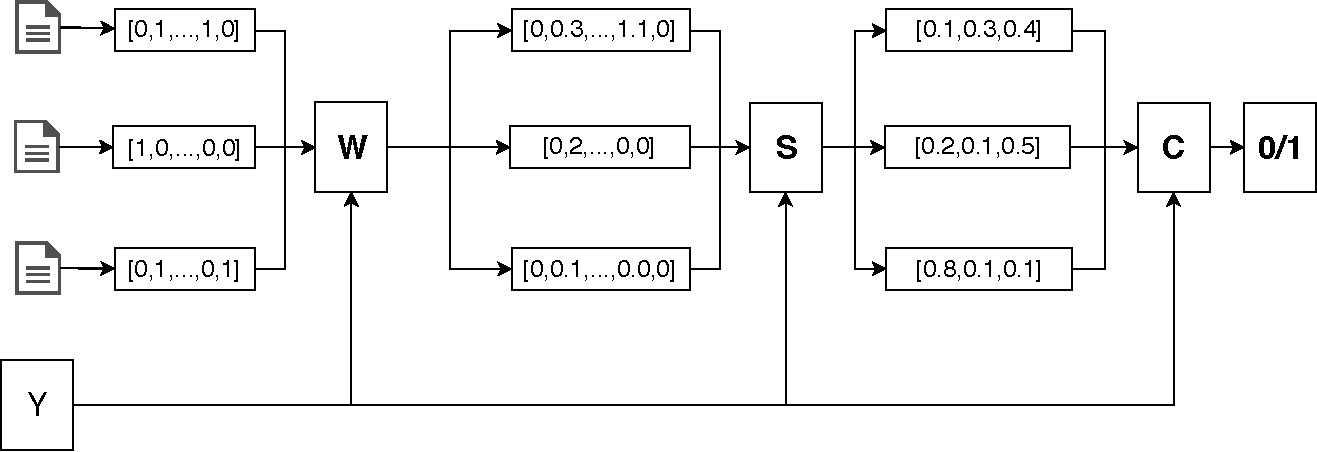
\includegraphics[width=0.9\textwidth]{LSA+supervision.pdf}
    \begin{block}
        
        $W$: reweighting

        $S$: decomposition
        
        $C$: classifier
    \end{block}
\end{frame}

\section{Our work}
\begin{frame}{eLSA}
    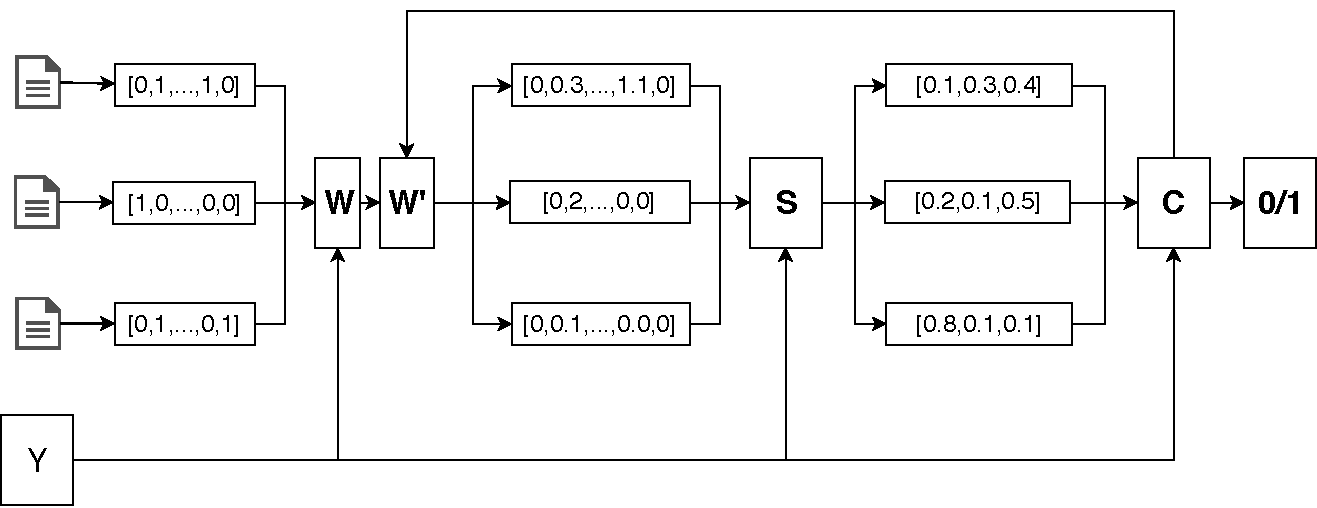
\includegraphics[width=0.9\textwidth]{eLSA.pdf}

    \begin{block}{eLSA}
        \begin{itemize}
            \item Apply weighting scheme $w$, rescale with $w'$, factorize, predict 
            \item Training the predictor, optimize $w'$
        \end{itemize}
    \end{block}
    
    LSA used in similar manner in \cite{ionescu2015training}
\end{frame} 


\begin{frame}{Gradient descent}
    \begin{columns}
    \column{0.5\linewidth}
    \begin{itemize}
        \item Co-occurrence matrix $M$
        \item Weight vector $w'$
    \end{itemize}
    \column{0.5\linewidth}
    \begin{itemize}
        \item SVD: $U \Sigma V^T$
        \item Simple classifier: $\sigma (v \theta + b)$
    \end{itemize}
    \end{columns}

    \begin{block}{}
    \begin{itemize}
        \item Reweighted matrix $M \circ w'$
        \item SVD decomposition $M \circ w' = U \Sigma V^T$
        \item Compute embedding $v = d \circ w' U$
        \item Train classifier $\hat{y} = \sigma (v \theta + b)$ to minimize $E = \frac{1}{2}(\hat{y}-y)^2$
        \item Compute derivative $\frac{\partial E}{\partial w'} = (\hat{y} -y) \hat{y} (1-\hat{y})\Theta U$
        \item Update weights: $w' = w' - \alpha \frac{\partial E}{\partial w'}$
    \end{itemize}    
    \end{block}
\end{frame} 

\section{Results}
\begin{frame}{Evaluation}
    \begin{block}{Datasets from SentEval \cite{conneau2017supervised}}
        \begin{itemize}
            \item Customer review dataset (CR)
            \item Movie review (MR)
            \item Subjective vs objective (SUBJ)
            \item Opinion polarity (MPQA)
            \item Questions types (TREC), actually $6$ datasets
        \end{itemize}
    \end{block}
    
\end{frame} 


\begin{frame}{eLSA learning curves}
    \begin{figure}
    \centerline{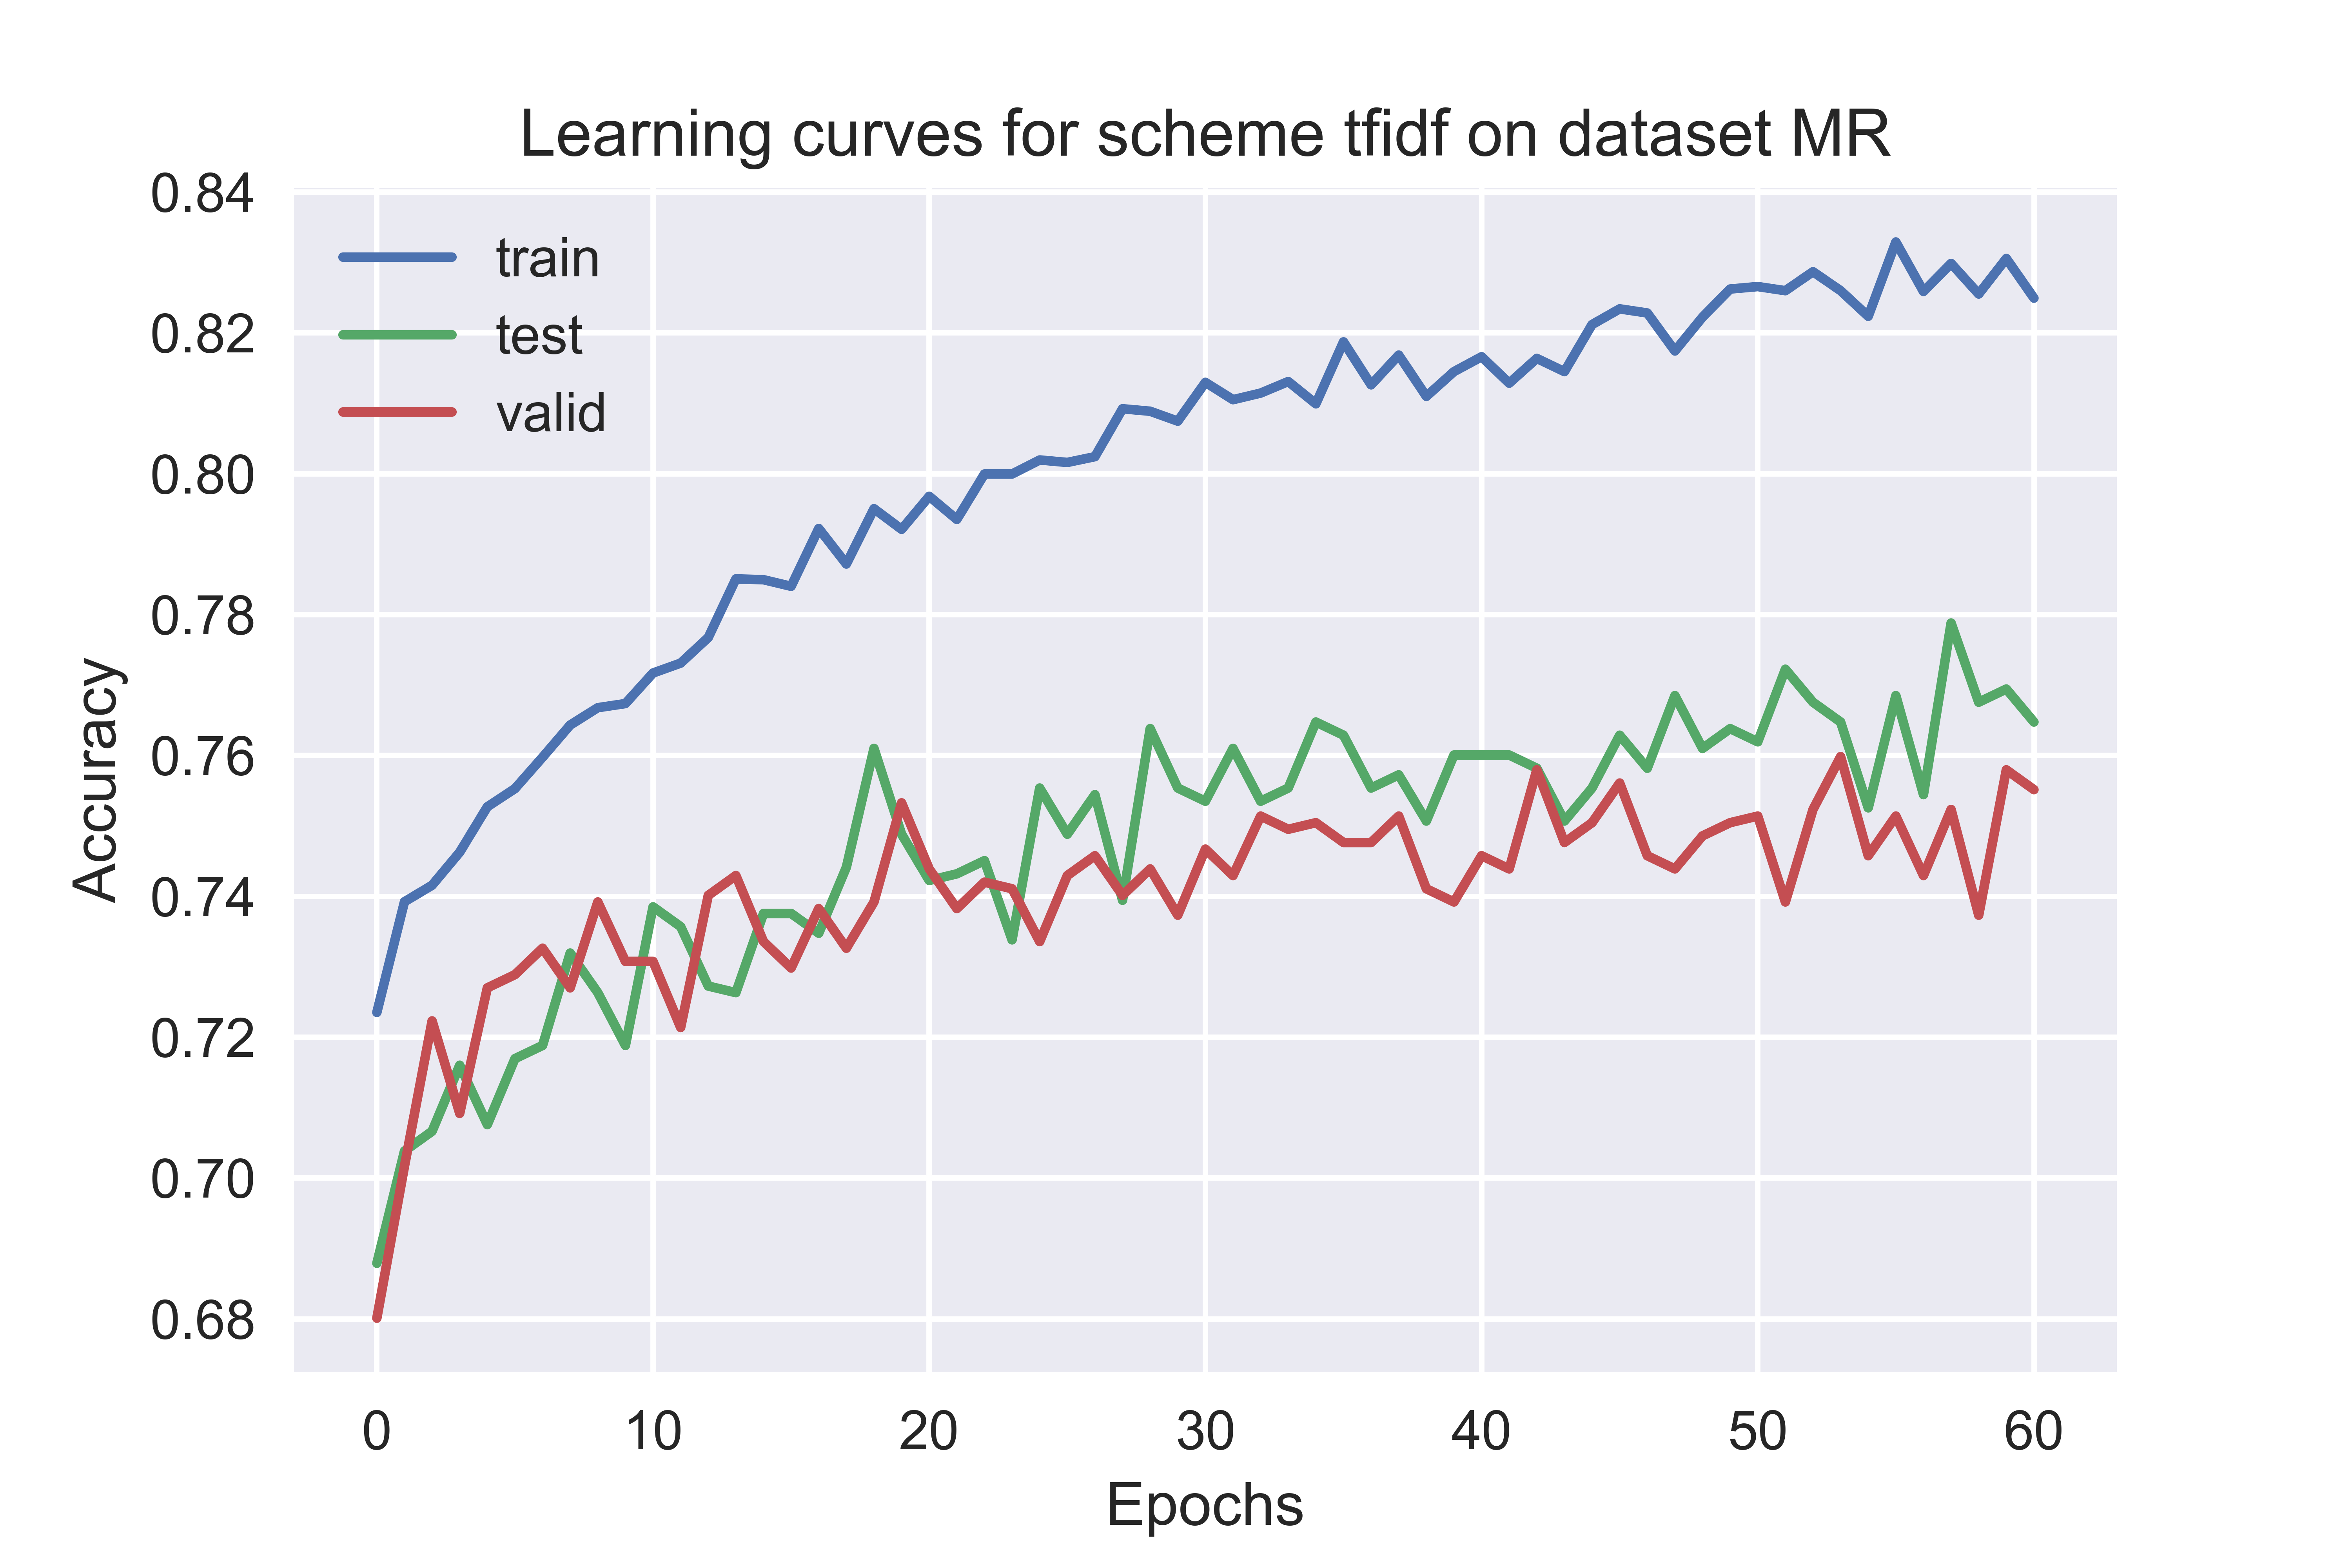
\includegraphics[width=0.8\textwidth]{learning_curve_MR_tfidf}}
    \caption[Learning curve for eLSA with tfidf weights on MR dataset]{Learning curve for eLSA with TFIDF weights on MR dataset}
    \label{img:learning:curve}
    \end{figure}
\end{frame} 

\begin{frame}{eLSA results}
    \small
\begin{table}[H]
\begin{center}

\begin{tabular}{ll|rrrr}
\toprule
   &   &   CR &  MPQA &   MR &  SUBJ \\
scheme & lsa &        &        &        &        \\
\midrule
None & 200 & \textbf{0.01} & \textbf{0.02} & \textbf{0.06} & \textbf{0.02} \\
   & 300 & \textbf{0.02} & \textbf{0.02} & \textbf{0.05} &     -0.0 \\
   & 400 & \textbf{0.03} & \textbf{0.01} & \textbf{0.04} & \textbf{0.01} \\
tfchi2 & 200 & \textbf{0.01} &      0.0 & \textbf{0.01} & \textbf{0.01} \\
   & 300 &      0.0 &     -0.0 & \textbf{0.02} & \textbf{0.01} \\
   & 400 & \textbf{0.01} &      0.0 & \textbf{0.03} & \textbf{0.02} \\
tfgr & 200 & \textbf{0.01} &     -0.0 & \textbf{0.01} & \textbf{0.02} \\
   & 300 & \textbf{0.01} &     -0.0 & \textbf{0.01} & \textbf{0.01} \\
   & 400 & \textbf{0.03} & \textbf{0.01} & \textbf{0.01} & \textbf{0.02} \\
\bottomrule
\end{tabular}

\caption[Accuracy increase over LSA]{Accuracy increase over LSA}
\label{tab:batch:results}
\end{center}
\end{table}
\end{frame}

\begin{frame}{eLSA results}
    \small
\begin{table}[H]
\begin{center}

\begin{tabular}{ll|rrrr}
\toprule
   &   &   CR &  MPQA &   MR &  SUBJ \\
scheme & lsa &        &        &        &        \\
\midrule
tfidf & 200 & \textbf{0.04} & \textbf{0.06} & \textbf{0.07} & \textbf{0.01} \\
   & 300 &     -0.0 & \textbf{0.05} & \textbf{0.05} &      0.0 \\
   & 400 &     -0.01 & \textbf{0.03} & \textbf{0.02} & \textbf{0.01} \\
tfig & 200 &      0.0 & \textbf{0.01} & \textbf{0.01} &     -0.0 \\
   & 300 &      0.0 & \textbf{0.01} & \textbf{0.01} & \textbf{0.01} \\
   & 400 & \textbf{0.03} &      0.0 & \textbf{0.02} & \textbf{0.01} \\
tfor & 200 & \textbf{0.01} &      0.0 &      0.0 & \textbf{0.01} \\
   & 300 &      0.0 &      0.0 &     -0.0 &      0.0 \\
   & 400 &     -0.0 & \textbf{0.02} &     -0.03 & \textbf{0.01} \\
\bottomrule
\end{tabular}

\caption[Accuracy increase over LSA]{Accuracy increase over LSA}
\label{tab:batch:results}
\end{center}
\end{table}
\end{frame}


\begin{frame}[fragile]{Insight}
\small
\begin{table}[h]
    \centering
    \begin{minipage}{.4\linewidth}
      \centering
        \begin{tabular}{lr}
\toprule
words &  $w'$ \\
\midrule
   is &  6.25 \\
  how &  5.87 \\
 what &  3.73 \\
   in &  3.60 \\
 mean &  3.51 \\
   of &  3.10 \\
 come &  3.09 \\
 long &  2.96 \\
  for &  2.94 \\
  the &  2.39 \\
\bottomrule
\end{tabular}

      \subcaption{Words with highest $w'$}
    \end{minipage}
    \begin{minipage}{.4\linewidth}
      \centering
        \begin{tabular}{lr}
\toprule
        words &  $w'$ \\
\midrule
         from &  0.42 \\
          its &  0.41 \\
     nickname &  0.38 \\
      address &  0.34 \\
 abbreviation &  0.32 \\
         fast &  0.32 \\
         term &  0.25 \\
         word &  0.24 \\
      between &  0.04 \\
            ? &  0.00 \\
\bottomrule
\end{tabular}

      \subcaption{Words with lowest $w'$}
    \end{minipage} 
    \caption{Most reweighted words on DESC dataset for scheme TFIDF}
    \label{tab:words:trec:tfidf}
\end{table}
\end{frame}



\begin{frame}[fragile]{Insight}
\small
\begin{table}[H]
    \centering
    \begin{minipage}{.4\linewidth}
      \centering
        \begin{tabular}{lr}
\toprule
      words &  $w'$ \\
\midrule
         is &  7.69 \\
        are &  4.52 \\
       what &  3.52 \\
       mean &  3.44 \\
     origin &  3.42 \\
 difference &  3.20 \\
       much &  2.91 \\
       long &  2.79 \\
      where &  2.72 \\
 definition &  2.71 \\
\bottomrule
\end{tabular}

      \subcaption{Words with highest $w'$}
    \end{minipage}
    \begin{minipage}{.4\linewidth}
      \centering
        \begin{tabular}{lr}
\toprule
words &  $w'$ \\
\midrule
  out &  1.00 \\
 name &  0.98 \\
  you &  0.97 \\
 does &  0.93 \\
   in &  0.90 \\
  who &  0.83 \\
   do &  0.71 \\
    ? &  0.59 \\
  was &  0.46 \\
  the &  0.00 \\
\bottomrule
\end{tabular}

      \subcaption{Words with lowest $w'$}
    \end{minipage} 
    \caption{Most reweighted words on DESC dataset for scheme TFIG}
    \label{tab:words:TREC:tfig}
\end{table}
\end{frame}





\begin{frame}{Other experiments}
    \begin{itemize}
        \item word vectors baselines
        \item learning rates for $w'$
        \item batch gradient descent
        \item stochastic gradient descent
        \item even more datasets
    \end{itemize}
\end{frame} 

\subsection{Literature}                
\begin{frame}[allowframebreaks]{Literature}
\footnotesize
    \nocite{*}
    \bibliographystyle{apalike}
    \bibliography{prezentacia.bib} 
\end{frame}

\begin{frame}
    \vfill
    \begin{center}
        \huge\bfseries
        Thank you for your attention
        \vfill
    \end{center}
    \vfill
\end{frame}

\appendix

%\item "SVD dekompozíciu považoval pri počítaní grandientu za konštantu a nie funkciu vektora váh" "iba okrajovo túto možnosť spomína"
% SRSLY!!?!? cela kapitola v related work, a udavame presne dvovody preco


\begin{frame}{Opponent's review}
    \begin{block}{Notation}
        \begin{itemize}   
            \item ``označenia bez akéhokoľvek vysvetlenia''
            \item ``matica M'' % pre čitateľa má byť podstatné len to, že to je matica dokumentov. Používame maticu MT, lebo je to z nejakheho dvovodu standard pre robenie SVD dekompozicie.
            \item ``SVD ako konštanta''

            \item ``documenty alebo vety'': ``We consider the sentences to be basically identical to documents as they both
can be considered to be sequences of words.''        
             
        \end{itemize}
    \end{block}
\end{frame} 

\begin{frame}{Opponent's review}
    \begin{block}{Bibliography}
        \begin{itemize}   
            \item 62 citations on 6 pages
            \item researched other thesis (Vajdová, 2017)
            \item stochastic gradient descent: [19] \cite{Goodfellow-et-al-2016},  [8] \cite{bottou-bousquet-2008},
            [55] \cite{rumelhart1986david},  % powered by maria vajdova
            \item TF-IDF: [56], \cite{salton1988term}
        \end{itemize}
    \end{block}
\end{frame} 

\begin{frame}{Opponent's review}
    \begin{block}{Weighting schemes}
        \begin{itemize}   
            \item Weighting  schemes [61] [29] [18]
        \end{itemize}
    \end{block}
    
    \begin{align*}
        ig = &\frac{a}{N}\log_2{\frac{aN}{(a+b)(a+c)}} + \frac{b}{N}\log_2{\frac{bN}{(a+b)(b+d)}} + \\ &\frac{c}{N}\log_2{\frac{cN}{(a+c)(c+d)}} + \frac{d}{N}\log_2{\frac{dN}{(b+d)(c+d)}} \\
    \end{align*}
    $$gr=\frac{ig}{-\frac{a+b}{N}\log_2{\frac{a+b}{N}} - \frac{c+d}{N}\log_2{\frac{c+d}{N}}}$$
    
    
\end{frame} 

\begin{frame}{Opponent's review}
    \begin{block}{Default model parameters}
        \begin{itemize}   
            \item mentioned the relevant ones
            \item others: \textbf{penalty}, dual, tol, C, fit\_intercept, intercept\_scaling, class\_weight, random\_state, solver, max\_iter, multi\_class, warm\_start, \textbf{kernel}, degree, gamma, coef0, shrinking, probability, cache\_size, decision\_function\_shape, alpha, window, min\_count, sample, seed, workers, min\_alpha, sg, hs, negative, cbow\_mean, hashfxn, iter, null\_word, trim\_rule, sorted\_vocab, batch\_words, compute\_loss, callbacks, num\_topics, id2word, chunksize, decay, distributed, onepass, power\_iters, extra\_samples
        \end{itemize}
    \end{block}
\end{frame} 

\begin{frame}{Opponent's review}
    \begin{block}{Others}
        \begin{itemize}   
            \item ``Ako sa spoja TF a IDF váhy do jednej'': multiplication
            \item Classifier in 4.2.3: logistic regression % we used SVM as well, but results were poor, multiple classifiers should be changed to logistic regression
        \end{itemize}
    \end{block}
\end{frame} 

\begin{frame}{Opponent's questions}
    \small
    \begin{block}{Constrains on $w'$}
        \begin{itemize}
            \itemsep0em
            \item We tried regularization, but results were poor
            \item Other constrains are extremely hard (GANS)
            \item In practice, results were fine
        \end{itemize}
    \end{block}
    
    \begin{block}{$w'$ vs $2w'$}
        \begin{itemize}
            \itemsep0em
            \item In theory, no difference % SVD should be the same, it should be absorbed in the classifiers weights.
            \item In practice the classifier may be regularized
            \item Experimentally, weights are centered around 1 (4.4.1.2)
        \end{itemize}
    \end{block}
    
    \begin{block}{Underweighting vs overweighting}
        \begin{itemize}
            \itemsep0em
            \item Relative change in ordering % what we did
            \item Notions of importance % Ze momentalne existuje niekolko sposobov, ako zistovat dvolezitost vstupu pre klasifikator, to by sa dalo aj tu.
            %\item Kombinácia týchto čísel by len bola arbitrary číslo 4.21 a 4.22
        \end{itemize}
    \end{block}
\end{frame}

\begin{frame}{Supervisor's review}
    \begin{block}{Datasets}
        \begin{itemize}
            \item Customer review dataset (CR)
            \item Movie review (MR)
            \item Subjective vs objective (SUBJ)
            \item Opinion polarity (MPQA)
            \item Questions types (TREC)
            \begin{itemize}
                \item ABBR  
                \item DESC  
                \item ENTY  
                \item HUM   
                \item LOC  
                \item NUM
            \end{itemize}
        \end{itemize}            
    \end{block}
\end{frame}

\begin{frame}{Supervisor's review}
    \begin{block}{Time complexity}
        \begin{itemize}
            \item LSA: $1-3$, complexity depends on SVD
            \item eLSA: $LSA \times epochs$, (35)
            \item word2vec: $5$, $C \times (D + D \times \log_2(V))$
        \end{itemize}
    \end{block}
\end{frame}



\begin{frame}{Count vs. prediction}
    \begin{block}{Prediction}
        \begin{itemize}
            \item extremely popular
            \item huge performance gains
            \item less memory demanding
        \end{itemize}
    \end{block}

    \begin{block}{Count}
        \begin{itemize}
            \item less hyperparameters
            \item easier to ``train''
            \item teoreticaly based
        \end{itemize}
    \end{block}
\end{frame}

\begin{frame}{Count vs prediction}
    \begin{block}{Glove vectors as explicit factorization}
        \begin{itemize}
            \item Neural word embedding as implicit matrix factorization \cite{levy2014neural}
        \end{itemize}
    \end{block}

    \begin{block}{Hyperparameters matter}
        \begin{itemize}
            \item Improving distributional similarity with lessons learned from word embeddings \cite{levy2015improving}
        \end{itemize}
    \end{block}

    \begin{block}{Does not work well on small datasets}
        \begin{itemize}
            \item Comparative study of LSA vs Word2vec embeddings in small corpora \cite{altszyler2016comparative}
        \end{itemize}
    \end{block}
\end{frame} 


% vocabulary!
%have
%restrictive
%word
%and/end/ant
%problematics
%embedding

%fixni grafy: osi + legenda



\end{document}\grid
